\documentclass[a4paper]{article} 
\usepackage{tcolorbox}
\tcbuselibrary{skins}

\title{
\vspace{-3em}
\begin{tcolorbox}[colframe=white,opacityback=0]
\begin{tcolorbox}
\Huge\sffamily Language of Composition 4$-$7
\end{tcolorbox}
\end{tcolorbox}
\vspace{-3em}
}

\date{}

\usepackage{background}
\SetBgScale{1}
\SetBgAngle{0}
\SetBgColor{grey}
\SetBgContents{\rule[0em]{4pt}{\textheight}}
\SetBgHshift{-2.3cm}
\SetBgVshift{0cm}

\usepackage{lipsum}% just to generate filler text for the example
\usepackage[margin=2cm]{geometry}

\usepackage{tikz}
\usepackage{tikzpagenodes}

\parindent=0pt

\usepackage{xparse}
\DeclareDocumentCommand\topic{ m m g g g g g}
{
\begin{tcolorbox}[sidebyside,sidebyside align=top,opacityframe=0,opacityback=0,opacitybacktitle=0, opacitytext=1,lefthand width=.3\textwidth]
\begin{tcolorbox}[colback=red!05,colframe=red!25,sidebyside align=top,width=\textwidth,before skip=0pt]
#1.\end{tcolorbox}%
\tcblower
\begin{tcolorbox}[colback=blue!05,colframe=blue!10,width=\textwidth,before skip=0pt]
#2
\end{tcolorbox}
\IfNoValueF {#3}{
\begin{tcolorbox}[colback=blue!05,colframe=blue!10,width=\textwidth]
#3
\end{tcolorbox}
}
\IfNoValueF {#4}{
\begin{tcolorbox}[colback=blue!05,colframe=blue!10,width=\textwidth]
#4
\end{tcolorbox}
}
\IfNoValueF {#5}{
\begin{tcolorbox}[colback=blue!05,colframe=blue!10,width=\textwidth]
#5
\end{tcolorbox}
}
\IfNoValueF {#6}{
\begin{tcolorbox}[colback=blue!05,colframe=blue!10,width=\textwidth]
#6
\end{tcolorbox}
}
\IfNoValueF {#7}{
\begin{tcolorbox}[colback=blue!05,colframe=blue!10,width=\textwidth]
#7
\end{tcolorbox}
}
\end{tcolorbox}
}

\def\summary#1{
\begin{tikzpicture}[overlay,remember picture,inner sep=0pt, outer sep=0pt]
\node[anchor=south,yshift=-1ex] at (current page text area.south) {% 
\begin{minipage}{\textwidth}%%%%
\begin{tcolorbox}[colframe=white,opacityback=0]
\begin{tcolorbox}[enhanced,colframe=black,fonttitle=\large\bfseries\sffamily,sidebyside=true, nobeforeafter,before=\vfil,after=\vfil,colupper=black,sidebyside align=top, lefthand width=.95\textwidth,opacitybacktitle=1, opacitytext=1,
segmentation style={black!55,solid,opacity=0,line width=3pt},
title=Summary
]
#1
\end{tcolorbox}
\end{tcolorbox}
\end{minipage}
};
\end{tikzpicture}
}

\usepackage{graphicx}
\usepackage{physics}
\usepackage{amsmath}
\usepackage{tikz}
\usepackage{mathdots}
\usepackage{yhmath}
\usepackage{cancel}
\usepackage{color}
\usepackage{siunitx}
\usepackage{array}
\usepackage{multirow}
\usepackage{amssymb}
\usepackage{gensymb}
\usepackage{tabularx}
\usepackage{booktabs}
\usetikzlibrary{fadings}
\usetikzlibrary{patterns}
\usetikzlibrary{shadows.blur}
\usetikzlibrary{shapes}

\begin{document} 
\maketitle

\topic{Exigence}{The need or demand. Why is \underline{NOW} the time \& place for a message}%

\topic{Rhetoric}{The ability to discern the available means of persuasion in any given situation.}%

\topic{Visual Rhetoric}{``Writing with images'' Ex. documentaries, illustrations, advertisements, cartoons, etc.}%

\topic{Audience}{A group to whom a work is meant to be presented to. Must establish what the viewer's values or morals are in order to have an effective message}%

\topic{Text}{Products meant to be read}%

\topic{Context}{Parts of discourse that surround a word or passage}%

\topic{Rhetorical Triangle}{A way to conceptualize the relationship between elements of a text}%

\summary{\centering\tikzset{every picture/.style={line width=0.75pt}} %set default line width to 0.75pt        

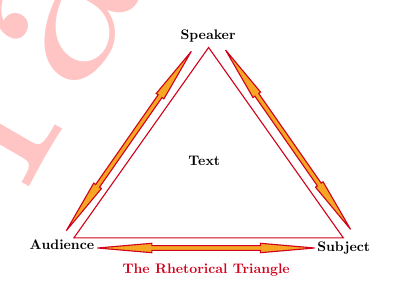
\begin{tikzpicture}[x=0.75pt,y=0.75pt,yscale=-.5,xscale=.5]
%uncomment if require: \path (0,374); %set diagram left start at 0, and has height of 374

%Shape: Triangle [id:dp3926678547967024] 
\draw  [color={rgb, 255:red, 208; green, 2; blue, 27 }  ,draw opacity=1 ][fill={rgb, 255:red, 255; green, 255; blue, 255 }  ,fill opacity=1 ] (326.32,82.68) -- (456.15,266.17) -- (196.49,266.17) -- cycle ;
%Left Right Arrow [id:dp19943991138135786] 
\draw  [color={rgb, 255:red, 208; green, 2; blue, 27 }  ,draw opacity=1 ][fill={rgb, 255:red, 245; green, 166; blue, 35 }  ,fill opacity=1 ] (219.28,275.9) -- (271.6,271.36) -- (271.6,273.63) -- (376.23,273.63) -- (376.23,271.36) -- (428.54,275.9) -- (376.23,280.43) -- (376.23,278.16) -- (271.6,278.16) -- (271.6,280.43) -- cycle ;
%Left Right Arrow [id:dp20777623482608543] 
\draw  [color={rgb, 255:red, 208; green, 2; blue, 27 }  ,draw opacity=1 ][fill={rgb, 255:red, 245; green, 166; blue, 35 }  ,fill opacity=1 ] (189.21,259.22) -- (215.64,213.39) -- (217.49,214.7) -- (277.73,128.29) -- (275.88,126.97) -- (309.69,86.39) -- (283.26,132.22) -- (281.41,130.91) -- (221.18,217.32) -- (223.02,218.64) -- cycle ;
%Left Right Arrow [id:dp7601860485249441] 
\draw  [color={rgb, 255:red, 208; green, 2; blue, 27 }  ,draw opacity=1 ][fill={rgb, 255:red, 245; green, 166; blue, 35 }  ,fill opacity=1 ] (463.11,257.92) -- (436.64,212.11) -- (434.82,213.41) -- (374.58,127) -- (376.41,125.7) -- (342.63,85.09) -- (369.09,130.9) -- (370.92,129.6) -- (431.16,216.02) -- (429.33,217.32) -- cycle ;


% Text Node
\draw (305.67,186.02) node [anchor=north west][inner sep=0.75pt]  [xscale=0.5,yscale=0.5] [align=left] {\textbf{Text}};
% Text Node
\draw (152.51,267.07) node [anchor=north west][inner sep=0.75pt]  [xscale=0.5,yscale=0.5] [align=left] {\textbf{Audience}};
% Text Node
\draw (429.75,268.37) node [anchor=north west][inner sep=0.75pt]  [xscale=0.5,yscale=0.5] [align=left] {\textbf{Subject}};
% Text Node
\draw (298.08,64.13) node [anchor=north west][inner sep=0.75pt]  [xscale=0.5,yscale=0.5] [align=left] {\textbf{Speaker}};
% Text Node
\draw (242.16,290.41) node [anchor=north west][inner sep=0.75pt]  [xscale=0.5,yscale=0.5] [align=left] {\textbf{\textcolor[rgb]{0.82,0.01,0.11}{The Rhetorical Triangle}}};


\end{tikzpicture}
}

\newpage

\topic{Occasion}{Specific circumstances surrounding the creation of a text}%

\topic{Purpose}{The goal an author intends to achieve}%

\topic{Speaker}{The author of the text}%

\topic{Persona}{The difference between the speaker on and off stage}%

\topic{Subject}{The topic of the text}%

\topic{Ethos}{Greek word for character. Expertise, knowledge, sincerity. Conveys shared values}%

\topic{Pathos}{Emotions, desires, hopes, fears, prejudices. Rests with connotations}%

\topic{Logos}{Clear rational ideas, backed with statistics, examples, or details. Logic}%

\summary{Political campaigns often use pathos, rather than logos, in order to obtain a larger following}

%\topic{Here's another question to begin the new page.}{\lipsum[3]}%
%{\lipsum[4]}%
%{\lipsum[5]}%

%\summary{And another summary that will float to the bottom of the next page.}

\end{document}
